\documentclass[11pt]{amsart}
\usepackage[margin=1.15in]{geometry}
\usepackage{amssymb,amsmath,mathtools}
\usepackage{graphicx,booktabs,array}
\usepackage[hidelinks]{hyperref}
\usepackage[expansion=false]{microtype}

\newtheorem{theorem}{Theorem}[section]
\newtheorem{proposition}[theorem]{Proposition}
\newtheorem{lemma}[theorem]{Lemma}
\newtheorem{corollary}[theorem]{Corollary}
\newtheorem{mainthm}{Theorem}
\renewcommand{\themainthm}{\Alph{mainthm}}
\theoremstyle{definition}
\newtheorem{definition}[theorem]{Definition}
\newtheorem{remark}[theorem]{Remark}
\newtheorem{example}[theorem]{Example}

\newcommand{\ZZ}{\mathbb{Z}}
\newcommand{\QQ}{\mathbb{Q}}
\newcommand{\CC}{\mathbb{C}}
\newcommand{\e}{\mathbf e}
\newcommand{\vt}{\vartheta}
\newcommand{\cB}{\mathcal B}
\newcommand{\cC}{\mathcal C}
\newcommand{\bin}[2]{\binom{#1}{#2}}
\newcommand{\coef}[2]{\big[#1\big]_{#2}}
\newcommand{\zenodoDOI}{10.5281/zenodo.24122363}

\setlength{\emergencystretch}{2.5em}
\hbadness=2000
\raggedbottom
\begin{document}

\title[Positive degeneracies for higher torsion dyons]{Positive Black Hole Degeneracies\\ for Dyons of Higher Torsion}

\author{Deep Bhattacharjee}
\address{Formerly, Electro-Gravitational Space Propulsion Laboratory (EGSPL), Bhubaneswar, Odisha 751030, India}
\address{Formerly, University of Calcutta (Heramba Chandra College), 23/49 Gariahat Road, Golpark, Kolkata 700029, West Bengal, India}
\email{d.bhattacharjee@erl-forschung.de}
\email{itsdeep@live.com}
\email{egspl@proton.me (GitHub-related contact; GitHub account creelie)}
\urladdr{https://orcid.org/0000-0003-0466-750X}

\begin{abstract}
Sen's argument says that a single-centred quarter-BPS black hole carries a positive index. For dyons of torsion $r>1$ in string theory on $K3\times T^2$ we prove this for every $r$ when the magnetic charge has $P^2/2=1$ or $2$. For every magnetic charge, odd torsion follows from the primitive case and even torsion from one inequality between primitive indices.

\medskip\noindent\textbf{Keywords:} black hole degeneracies; non-primitive dyons; mock Jacobi forms.

\smallskip\noindent\textbf{MSC 2020:} 11F50 (primary); 11F37, 11P82, 81T30, 83E30.
\end{abstract}

\maketitle

\section{Introduction}\label{sec:intro}

A quarter-BPS dyon of $\mathcal N=4$ string theory in four dimensions carries an electric charge vector $Q$ and a magnetic charge vector $P$ in the Narain lattice $\Gamma^{22,6}$, and its protected index is a sixth helicity supertrace. When the charges support a single-centred black hole, Sen observed that the only states not belonging to the horizon are the zero modes of the broken supersymmetries, and that the spherical symmetry of the horizon then forces the horizon states to be bosonic \cite{Sen11}. The index of a single-centred black hole, normalised so as to strip off the fermion zero modes, must therefore be positive.\footnote{The argument and the normalisation are explained in Sections~1 and~2 of \cite{Sen11}. The relation between the index and the entropy of the black hole goes back to the entropy function formalism reviewed in \cite{Sen08}, and the relation between index and degeneracy for supersymmetric black holes is derived in \cite{DGMS11}. In frames where the classical solution carries hair outside the horizon one must first remove the hair; for type~II string theory on $K3\times T^2$ in the heterotic frame no further hair is present, see \cite{CD21}.} On the microscopic side the index is a Fourier coefficient of the inverse of a Siegel modular form, and the conjecture becomes a statement about the signs of these coefficients.

For charges of torsion one, that is with $\gcd(Q\wedge P)=1$, the partition function is the inverse of the Igusa cusp form $\Phi_{10}$ \cite{DVV97,SSY06}. Dabholkar, Murthy and Zagier showed that, once the contribution of two-centred bound states is removed, the generating function of the single-centred indices of magnetic charge $m=P^2/2$ is a mock Jacobi form $\psi^F_m$; Bringmann and Murthy used explicit formulas for $\psi^F_1$ and $\psi^F_2$ to prove the positivity conjecture for $m=1$ and $m=2$ and every electric charge \cite{BM13}.\footnote{A review of these mock Jacobi forms and their role in black hole counting is \cite{Mur25}. The construction of $\Phi_{10}$ as an automorphic correction of a Lorentzian Kac--Moody algebra is in \cite{GN97}.}

Most charges are not primitive. A dyon has torsion $r=\gcd(Q\wedge P)$, the greatest common divisor of the $2\times2$ minors $Q_iP_j-Q_jP_i$, and for $r>1$ the partition function is no longer $1/\Phi_{10}$. Banerjee, Sen and Srivastava proposed the partition function of the family $\cB_r$ of dyons with $Q$ equal to $r$ times a primitive vector \cite{BSS08a,BSS08b}, and Dabholkar, Gomes and Murthy derived the same formula from the microscopic theory \cite{DGM11}. The index of a dyon of torsion $r$ is a weighted sum of indices of torsion one with the weights $s$ running over the divisors of $r$, and with signs. The signs are the whole difficulty: for even $r$ some of the terms are negative, so positivity of the primitive indices does not by itself give positivity at torsion $r$. As far as we know the sign of the single-centred index at torsion $r>1$ has not been settled for any family of charges.

Write $n=Q^2/2$, $\ell=Q\cdot P$, $m=P^2/2$ and $\Delta=4mn-\ell^2=Q^2P^2-(Q\cdot P)^2$. Let $d^*_r(Q,P)$ be the index of a dyon $(Q,P)\in\cB_r$ computed with Sen's attractor contour (Definition~\ref{def:dstar}). Our main result is the following.

\begin{mainthm}\label{thm:A}
Let $r\ge1$ and let $(Q,P)\in\cB_r$ with $P^2/2\in\{1,2\}$ and $Q^2P^2-(Q\cdot P)^2>0$. Then $d^*_r(Q,P)>0$.
\end{mainthm}

The proof has two parts. The first is a reduction that holds for every magnetic charge.

\begin{mainthm}\label{thm:B}
Fix $m\ge1$ and assume that the single-centred index of torsion one satisfies $d^*(n',\ell',m)>0$ whenever $4mn'-\ell'^2>0$. Then $d^*_r(Q,P)>0$ for every odd $r$ and every $(Q,P)\in\cB_r$ with $P^2/2=m$ and $\Delta>0$. If in addition
\begin{equation}\label{eq:doubling}
d^*(4n',2\ell',m)>2\,d^*(n',\ell',m)\qquad\text{for all $\ell'$ odd with } 4mn'-\ell'^2>0,
\end{equation}
then $d^*_r(Q,P)>0$ for every $r\ge1$.
\end{mainthm}

The second part proves the doubling inequality \eqref{eq:doubling} for $m=1$ and $m=2$.

\begin{mainthm}\label{thm:C}
The doubling inequality \eqref{eq:doubling} holds for $m=1$ and for $m=2$.
\end{mainthm}

Theorem~\ref{thm:A} follows from Theorems~\ref{thm:B} and~\ref{thm:C} together with the positivity of the primitive indices for $m=1,2$ proved in \cite{BM13}.

The idea behind Theorem~\ref{thm:B} is a pairing. In the torsion sum the term of a divisor $s$ is negative only when $s$ is even and $\ell/s$ is odd, and then the term of $s/2$ is positive and involves the charge $(4n/s^2,2\ell/s,m)$, whose discriminant is four times that of the negative term. Since the single-centred index grows like $\exp(\pi\sqrt{\Delta})$, quadrupling the discriminant doubles the exponent, and one expects \eqref{eq:doubling} to hold with an enormous margin. Figure~\ref{fig:doubling} shows that the ratio of the two sides of \eqref{eq:doubling} is at least $325$ in every case we computed, and grows quickly with the discriminant.

The proof of Theorem~\ref{thm:C} is elementary. We write the two sides of \eqref{eq:doubling} through the $q$-series of Bringmann and Murthy, drop the class number terms in the direction that weakens the inequality, and compare the remaining coefficients through two facts about coloured partitions: the bound $p_k(N+1)\le(k+1)\,p_k(N)$ for the number of $k$-coloured partitions, and the factorisation $(q;q)_\infty^{-k}=\Psi(q)^k\,(q^4;q^4)_\infty^{-k}$, where $\Psi$ counts partitions into parts not divisible by four. The factorisation matches the coefficient of $q^{4N}$ on the left of \eqref{eq:doubling} with the coefficient of $q^N$ on the right term by term, and the remaining estimates are explicit inequalities between binomial coefficients and divisor sums. A finite table of exact values covers the smallest discriminants: $D'\le 31$ for $m=1$ and $D'\le 39$ for $m=2$, where $D'$ is the discriminant of the negative term.

The paper is organised as follows. Section~\ref{sec:setup} recalls the partition functions and derives the torsion formula for the single-centred index with its signs. Section~\ref{sec:reduction} proves Theorem~\ref{thm:B}. Section~\ref{sec:partitions} contains the two partition lemmas. Sections~\ref{sec:m1} and~\ref{sec:m2} prove the doubling inequality for $m=1$ and $m=2$, and Section~\ref{sec:proofA} completes the proof of Theorem~\ref{thm:A} and discusses general $m$. Appendix~\ref{app:qseries} derives the $q$-series from the formulas of \cite{BM13}, Appendix~\ref{app:bounds} proves the coefficient bounds, and Appendix~\ref{app:tables} lists the exact values used.

\subsection*{Notation}
We write $q=e^{2\pi i\tau}$, $\e(x)=e^{2\pi ix}$ and $(q;q)_\infty=\prod_{j\ge1}(1-q^j)$. For a power series $F=\sum a(j)q^j$ we write $\coef{F}{j}=a(j)$, with $\coef{F}{j}=0$ for $j<0$, and $F\succeq0$ when all coefficients are non-negative. For $k\ge1$ let
\[
P_k(q)=(q;q)_\infty^{-k}=\sum_{N\ge0}p_k(N)\,q^N,
\]
so that $p_k(N)$ is the number of $k$-coloured partitions of $N$. The Eisenstein series are $E_2=1-24\sum\sigma_1(j)q^j$, $E_4=1+240\sum\sigma_3(j)q^j$ and $E_6=1-504\sum\sigma_5(j)q^j$, the operator $D=q\,\frac{d}{dq}$ acts on $q$-series, and $H(N)$ is the Hurwitz class number, with $H(0)=-1/12$ and $H(N)>0$ for $N\ge1$ \cite{HZ76,Zag08}. We use the theta series
\[
\theta_0=\sum_{k\in\ZZ}q^{k^2},\qquad T=\sum_{k\ge0}q^{k(k+1)},\qquad V=\sum_{k\ge0}q^{k(k+1)/2}.
\]

\section{Charges, torsion and the single-centred index}\label{sec:setup}

\subsection{Torsion one}
Type~IIB string theory on $K3\times T^2$ is dual to the heterotic string on $T^6$, and in the heterotic frame the charges $(Q,P)$ of a dyon are a pair of vectors in the even unimodular lattice $\Gamma^{22,6}$.\footnote{For the heterotic string and its relation to M-theory see \cite{SBBT26}; for the geometry of $K3$ surfaces, their involutions and the $K3$-fibred Calabi--Yau threefolds behind the dual type~II descriptions see \cite{BN26,Bha22}.} The $T$-duality invariants are $n=Q^2/2$, $\ell=Q\cdot P$ and $m=P^2/2$, and for torsion one they determine the charges up to $T$-duality. The partition function is
\begin{equation}\label{eq:Phi10}
\frac1{\Phi_{10}(\tau,z,\tau')}=\sum_{m\ge-1}\psi_m(\tau,z)\,\e(m\tau'),
\end{equation}
where $\Phi_{10}$ is the Igusa cusp form of weight $10$ and $\psi_m$ is a meromorphic Jacobi form of weight $-10$ and index $m$ \cite{BM13}. The variables $\tau,z,\tau'$ are conjugate to $n,\ell,m$.

Because $\Phi_{10}$ vanishes on the divisor $z=0$ and its images, the Fourier coefficients of $1/\Phi_{10}$ depend on the imaginary parts of $(\tau,z,\tau')$. Following Sen \cite{Sen07,Sen11} and the contour prescription of Banerjee, Sen and Srivastava \cite{BSS09}, the single-centred index is the coefficient taken on the contour fixed by the attractor values of the moduli.\footnote{At the attractor point of the charges no two-centred bound state exists, so only the single-centred black hole contributes; see \cite{Sen07} and \cite{CV08} for the walls of marginal stability and the discrete attractor flow.}

\begin{definition}\label{def:dstar}
For $(n,\ell,m)$ with $\Delta=4mn-\ell^2>0$ let $\cC^*(n,\ell,m)$ be the contour
\[
0\le\operatorname{Re}\tau,\operatorname{Re}z,\operatorname{Re}\tau'\le1,\qquad \operatorname{Im}\tau=2m\Lambda,\quad \operatorname{Im}\tau'=2n\Lambda,\quad\operatorname{Im}z=-\ell\Lambda,
\]
with $\Lambda$ large, and put
\begin{equation}\label{eq:dstar1}
d^*(n,\ell,m)=(-1)^{\ell+1}\int_{\cC^*(n,\ell,m)}\frac{\e(-n\tau-\ell z-m\tau')}{\Phi_{10}(\tau,z,\tau')}\,d\tau\,dz\,d\tau'.
\end{equation}
For a dyon $(Q,P)$ of torsion one, $d^*(Q^2/2,Q\cdot P,P^2/2)$ is its single-centred index.
\end{definition}

The sign $(-1)^{\ell+1}$ accounts for the fermion zero modes and for the convention that counts bosonic minus fermionic supermultiplets \cite{BM13,Sen11}. Two properties of $d^*$ will be used. First, $d^*$ is invariant under the $S$-duality group $SL(2,\ZZ)$, which acts on $(n,\ell,m)$ as on the binary quadratic form $nx^2+\ell xy+my^2$: the attractor contour moves covariantly with the charges \cite{BSS09,Sen07}. In particular
\begin{equation}\label{eq:Sdual}
d^*(n,\ell,m)=d^*(n+k\ell+k^2m,\ \ell+2km,\ m)\quad(k\in\ZZ),\qquad d^*(n,\ell,m)=d^*(m,-\ell,n).
\end{equation}
Second, $d^*$ is a Fourier coefficient of a mock Jacobi form. Write $\psi_m=\psi_m^P+\psi_m^F$, where the polar part $\psi_m^P$ is the Appell--Lerch sum that carries the poles of $\psi_m$, and the finite part
\[
\psi^F_m(\tau,z)=\sum_{n,\ell}c^F_m(n,\ell)\,q^n\zeta^\ell,\qquad \zeta=\e(z),
\]
is a mock Jacobi form of index $m$. Dabholkar, Murthy and Zagier proved that the single-centred index is read off from $\psi^F_m$ \cite[Section~3.1]{BM13}: for a reduced triple, that is one with $|\ell|\le m\le n$,
\begin{equation}\label{eq:DMZ}
d^*(n,\ell,m)=(-1)^{\ell+1}c^F_m(n,\ell).
\end{equation}
The coefficients of $\psi^F_m$ satisfy the elliptic invariance of a Jacobi form of index $m$, so $c^F_m(n,\ell)$ depends only on $4mn-\ell^2$ and on $\ell$ modulo $2m$, and is even in $\ell$.

\begin{lemma}\label{lem:allcoeff}
Let $m\in\{1,2\}$. Then \eqref{eq:DMZ} holds for every $(n,\ell)$ with $4mn-\ell^2>0$.
\end{lemma}

\begin{proof}
Both sides of \eqref{eq:DMZ} are unchanged under $(n,\ell)\mapsto(n+k\ell+k^2m,\ell+2km)$, the left side by \eqref{eq:Sdual} and the right side by elliptic invariance; note that $(-1)^\ell$ is unchanged as well. Choosing $k$ we may assume $|\ell|\le m$. Since $4mn>\ell^2\ge0$ we have $n\ge1$. If $n\ge m$ the triple is reduced and \eqref{eq:DMZ} is the theorem quoted above. This settles $m=1$, and for $m=2$ leaves $n=1$ and $\ell\in\{0,\pm1,\pm2\}$. By \eqref{eq:Sdual}, $d^*(1,\ell,2)=d^*(2,-\ell,1)$, and the right side equals $(-1)^{\ell+1}c^F_1(2,\ell)$ by the case $m=1$. It remains to see that $c^F_2(1,\ell)=c^F_1(2,\ell)$ for $\ell=0,1,2$. Both sides are computed from the closed formulas \eqref{eq:psi1F} and \eqref{eq:psi2F} below; the values of $(-1)^{\ell+1}c^F$ are
\[
1127472,\qquad 561576,\qquad 50064
\]
for $\ell=0,1,2$ on either side (Appendix~\ref{app:tables}, Table~\ref{tab:prim}).\footnote{For $\ell=1,2$ this coincidence is noted in footnote~2 of \cite{BM13}; the case $\ell=0$ is the same check one coefficient further.}
\end{proof}

\subsection{\texorpdfstring{Torsion $r$}{Torsion r}}
Let $r\ge1$. Following \cite{BSS08a} let $\cB_r$ be the set of dyons $(Q,P)$ with $Q$ equal to $r$ times a primitive vector, $P$ primitive, and $Q/r$ and $P$ spanning a primitive sublattice of $\Gamma^{22,6}$. Such dyons have torsion $r$, two of them with the same invariants are related by $T$-duality, and the invariants satisfy
\begin{equation}\label{eq:quant}
\frac{Q^2}2\in r^2\ZZ,\qquad \frac{P^2}2\in\ZZ,\qquad Q\cdot P\in r\ZZ.
\end{equation}
Banerjee, Sen and Srivastava \cite[eqs.~(3)--(7)]{BSS08a} proposed, and Dabholkar, Gomes and Murthy derived from the microscopic conformal field theory \cite[eqs.~(3.24)--(3.28)]{DGM11}, the following formula for the index $d(Q,P)$ of a dyon in $\cB_r$:
\begin{equation}\label{eq:BSS}
d(Q,P)=(-1)^{Q\cdot P+1}\sum_{s\mid r}s\cdot s^3\int\frac{\e\big(-\tfrac12(\check\sigma Q^2+\check\rho P^2+2\check vQ\cdot P)\big)}{\Phi_{10}(\check\rho,s^2\check\sigma,s\check v)}\,d\check\rho\,d\check\sigma\,d\check v,
\end{equation}
where the real parts run over $|\operatorname{Re}\check\rho|\le\frac12$, $|\operatorname{Re}\check\sigma|\le\frac1{2s^2}$, $|\operatorname{Re}\check v|\le\frac1{2s}$, and the imaginary parts are fixed in a region where the expansion converges.\footnote{The weight $s$ in \eqref{eq:BSS} is the function $g(s)=s$ of \cite{BSS08a}, which is fixed there by the wall crossing formula for decays into non-primitive half-BPS states. In \eqref{eq:BSS} the variable $\check\sigma$ is conjugate to $Q^2/2$, $\check\rho$ to $P^2/2$ and $\check v$ to $Q\cdot P$; in the notation \eqref{eq:Phi10} this is $(\check\rho,\check\sigma,\check v)=(\tau',\tau,z)$, and the factor $\frac12$ in the exponent turns $Q^2,P^2$ into $n,m$.} The single-centred index $d^*_r(Q,P)$ is \eqref{eq:BSS} with the imaginary parts placed on the attractor contour of $(Q,P)$, which in these variables reads
\begin{equation}\label{eq:attr}
\operatorname{Im}\check\rho=2n\Lambda,\qquad\operatorname{Im}\check\sigma=2m\Lambda,\qquad\operatorname{Im}\check v=-\ell\Lambda.
\end{equation}

\begin{proposition}\label{prop:torsion}
Let $(Q,P)\in\cB_r$ with invariants $(n,\ell,m)$ and $\Delta>0$. Then
\begin{equation}\label{eq:torsion}
d^*_r(Q,P)=\sum_{s\mid r}s\,(-1)^{\ell-\ell/s}\,d^*\Big(\frac n{s^2},\frac\ell s,m\Big).
\end{equation}
Every triple on the right has positive discriminant $\Delta/s^2$.
\end{proposition}

\begin{proof}
By \eqref{eq:quant}, $n/s^2$ and $\ell/s$ are integers for $s\mid r$. In the term of $s$ substitute $\sigma=s^2\check\sigma$, $v=s\check v$ and $\rho=\check\rho$. The Jacobian is $d\check\sigma\,d\check v=s^{-3}d\sigma\,dv$, which cancels $s^3$, and the real parts of $\sigma$ and $v$ now run over intervals of length one. The exponent becomes
\[
\check\sigma n+\check\rho m+\check v\ell=\sigma\frac n{s^2}+\rho m+v\frac\ell s,
\]
so the integral is the Fourier coefficient of $1/\Phi_{10}(\rho,\sigma,v)$ at the invariants $(n/s^2,\ell/s,m)$. The contour \eqref{eq:attr} becomes
\[
\operatorname{Im}\rho=2n\Lambda=2\frac n{s^2}\Lambda',\qquad \operatorname{Im}\sigma=2s^2m\Lambda=2m\Lambda',\qquad \operatorname{Im}v=-s\ell\Lambda=-\frac\ell s\Lambda'
\]
with $\Lambda'=s^2\Lambda$, which is the attractor contour of $(n/s^2,\ell/s,m)$ in Definition~\ref{def:dstar}. Hence the term of $s$ equals $s\,(-1)^{\ell+1}\cdot(-1)^{\ell/s+1}d^*(n/s^2,\ell/s,m)$, and $(-1)^{\ell+1}(-1)^{\ell/s+1}=(-1)^{\ell-\ell/s}$. Finally $4m(n/s^2)-(\ell/s)^2=\Delta/s^2$.
\end{proof}

\begin{remark}\label{rem:torsionone}
For $r=1$ the formula reduces to the identity, and for $r=2$ it reads $d^*_2=d^*(n,\ell,m)\pm2\,d^*(n/4,\ell/2,m)$, with the minus sign exactly when $\ell/2$ is odd. Without the sign, \eqref{eq:torsion} is equation~(3.28) of \cite{DGM11}; the sign comes from the factor $(-1)^{Q\cdot P+1}$ in \eqref{eq:BSS} against the factor $(-1)^{\ell/s+1}$ in \eqref{eq:dstar1}.
\end{remark}

Sen's argument applies to every single-centred black hole, so it predicts $d^*_r(Q,P)>0$ for every $(Q,P)\in\cB_r$ with $\Delta>0$. For $r=1$ and $m\in\{1,2\}$ this is the theorem of Bringmann and Murthy \cite{BM13}.

\section{The reduction}\label{sec:reduction}

\begin{lemma}\label{lem:signs}
Let $s\mid r$ and $\ell\in r\ZZ$. The sign $(-1)^{\ell-\ell/s}$ in \eqref{eq:torsion} is $-1$ if and only if $s$ is even and $\ell/s$ is odd. In that case the sign attached to $s/2$ is $+1$.
\end{lemma}

\begin{proof}
Write $\ell=s\cdot(\ell/s)$, so $\ell-\ell/s=(s-1)(\ell/s)$. If $s$ is odd this is even. If $s$ is even it has the parity of $\ell/s$. For the second claim, $\ell/(s/2)=2\ell/s$ is even and $\ell$ is even, so $\ell-\ell/(s/2)$ is even.
\end{proof}

\begin{proof}[Proof of Theorem~\ref{thm:B}]
Let $(Q,P)\in\cB_r$ with invariants $(n,\ell,m)$ and $\Delta>0$. Every triple in \eqref{eq:torsion} has positive discriminant, so by hypothesis every $d^*$ on the right is positive. If $r$ is odd every divisor is odd, all signs are $+1$ by Lemma~\ref{lem:signs}, and $d^*_r(Q,P)>0$.

Let $r$ be even and let $\mathcal N$ be the set of divisors $s$ of $r$ with $s$ even and $\ell/s$ odd. By Lemma~\ref{lem:signs} the map $s\mapsto s/2$ sends $\mathcal N$ injectively into the set of divisors with positive sign, and its image does not meet $\mathcal N$. For $s\in\mathcal N$ put $n'=n/s^2$, $\ell'=\ell/s$; then $\ell'$ is odd, $4mn'-\ell'^2=\Delta/s^2>0$, and the term of $s/2$ is
\[
\frac s2\,d^*\Big(\frac{4n}{s^2},\frac{2\ell}s,m\Big)=\frac s2\,d^*(4n',2\ell',m).
\]
By \eqref{eq:doubling}, the sum of the terms of $s$ and $s/2$ is
\[
\frac s2\,d^*(4n',2\ell',m)-s\,d^*(n',\ell',m)=\frac s2\Big(d^*(4n',2\ell',m)-2d^*(n',\ell',m)\Big)>0.
\]
The divisors not in $\mathcal N\cup\tfrac12\mathcal N$ carry positive terms. The divisor $s=1$ is never in $\mathcal N$, and if $1\in\frac12\mathcal N$ it is paired; in either case the sum is a non-empty sum of positive quantities, so $d^*_r(Q,P)>0$.
\end{proof}

\begin{figure}[t]
\centering
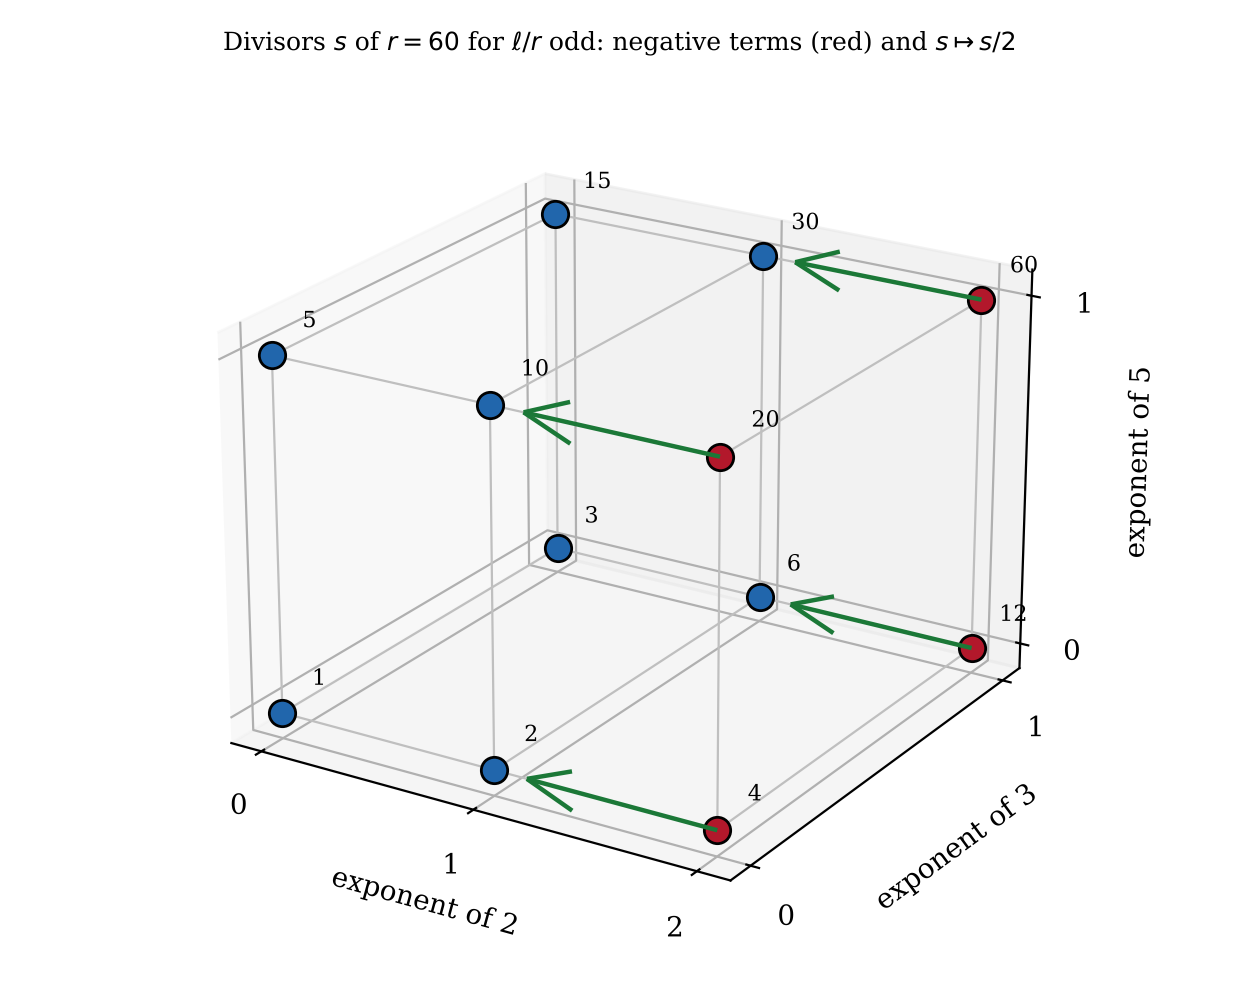
\includegraphics[width=0.72\textwidth]{figures/fig_pairing.png}
\caption{The divisors of $r=60$ arranged by their prime exponents. If $\ell/r$ is odd, then $\ell/s$ is odd exactly when $s$ contains the full power $4$ of $2$, so the negative terms of \eqref{eq:torsion} sit on the face where the exponent of $2$ is $2$ (red). Each is paired with $s/2$ on the adjacent face (arrows), whose term is positive and has four times the discriminant.}
\label{fig:pairing}
\end{figure}

\begin{remark}\label{rem:structure}
The pairing uses only the terms $s$ and $s/2$, and discards all other positive terms. Figure~\ref{fig:pairing} shows the pattern for $r=60$, and Figure~\ref{fig:terms} shows the sizes of the terms in three examples with $r=12$. The term $s=1$ dominates by many orders of magnitude, so \eqref{eq:doubling} is far from what positivity really needs; it is simply the cleanest sufficient condition.
\end{remark}

\begin{figure}[t]
\centering
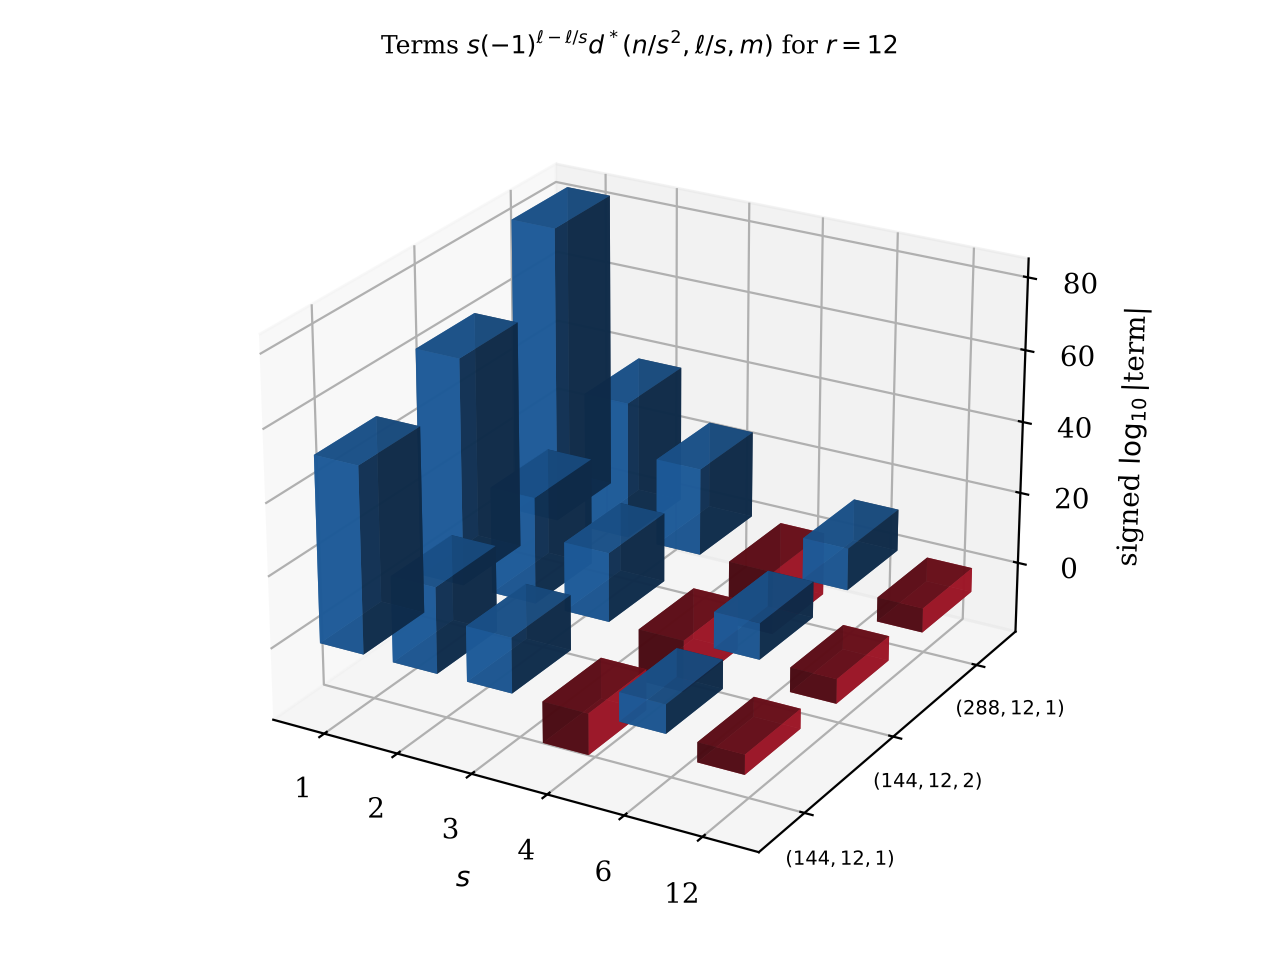
\includegraphics[width=0.74\textwidth]{figures/fig_terms.png}
\caption{Signed size $\pm\log_{10}|t_s|$ of the terms $t_s=s(-1)^{\ell-\ell/s}d^*(n/s^2,\ell/s,m)$ of \eqref{eq:torsion} for $r=12$ and the charges $(n,\ell,m)=(144,12,1)$, $(144,12,2)$ and $(288,12,1)$. Negative terms are red; they occur at $s=4$ and $s=12$, where $\ell/s$ is odd.}
\label{fig:terms}
\end{figure}

\section{Two lemmas on coloured partitions}\label{sec:partitions}

\begin{lemma}\label{lem:ratio}
For $k\ge1$ and $N\ge0$,
\[
p_k(N+1)\le(k+1)\,p_k(N),\qquad p_k(N)\ge\bin{N+k-1}{k-1},\qquad p_k(0)=1,\quad p_k(1)=k.
\]
\end{lemma}

\begin{proof}
A $k$-coloured partition of $N+1$ is a multiset of parts, each part a positive integer carrying one of $k$ colours. Split the $k$-coloured partitions $\lambda$ of $N+1$ into two classes. If $\lambda$ has a part equal to $1$, remove one part $1$ of the smallest colour that occurs among the parts $1$. The result is a partition of $N$, and $\lambda$ is recovered from it and the colour of the removed part, so this class has at most $k\,p_k(N)$ elements. If $\lambda$ has no part $1$, let $a\ge2$ be its smallest part and among the parts equal to $a$ choose one of the smallest colour $c$; replace it by $a-1$ of colour $c$. In the result the part $a-1$ is the unique smallest part, so $\lambda$ is recovered by raising it, and this class has at most $p_k(N)$ elements. Hence $p_k(N+1)\le(k+1)p_k(N)$.

For the lower bound, the partitions using only parts equal to $1$ already give $\binom{N+k-1}{k-1}$, the number of ways to distribute $N$ ones among $k$ colours. The values at $N=0,1$ are clear.
\end{proof}

\begin{lemma}\label{lem:dilation}
Let
\[
\Psi(q)=\frac{(q^4;q^4)_\infty}{(q;q)_\infty}=\prod_{4\nmid j}\frac1{1-q^j}.
\]
Then $\Psi^k\succeq(1-q)^{-k}$, so $\coef{\Psi^k}{M}\ge\binom{M+k-1}{k-1}$ for all $M\ge0$, with $\coef{\Psi^k}0=1$ and $\coef{\Psi^k}1=k$. Moreover
\begin{equation}\label{eq:dilation}
P_k(q)=\Psi(q)^k\,P_k(q^4),
\end{equation}
and for every power series $F$ and all integers $N\ge0$, $0\le a\le3$,
\begin{equation}\label{eq:dilcoef}
\coef{F\,P_k}{4N+a}=\sum_{i=-1}^{N}\coef{F\Psi^k}{4i+a}\,p_k(N-i),
\end{equation}
where the term $i=-1$ is present only when $4i+a\ge0$.
\end{lemma}

\begin{proof}
The product formula shows that $\Psi$ is the generating function of partitions into parts not divisible by $4$. Every $M\ge0$ has the partition into $M$ ones, so $\Psi\succeq(1-q)^{-1}$, and since both series have non-negative coefficients the same holds for the $k$-th powers. Identity \eqref{eq:dilation} is $(q;q)^{-k}=\big((q^4;q^4)/(q;q)\big)^k(q^4;q^4)^{-k}$. Since $P_k(q^4)=\sum_tp_k(t)q^{4t}$,
\[
\coef{F\Psi^kP_k(q^4)}{4N+a}=\sum_{t\ge0}\coef{F\Psi^k}{4N+a-4t}\,p_k(t),
\]
and the substitution $i=N-t$ gives \eqref{eq:dilcoef}; the index $i$ is at least $-1$ because $4i+a\ge0$ with $a\le3$.
\end{proof}

The point of \eqref{eq:dilcoef} is that the coefficient of $q^{4N}$ of a product with $P_k$ is expressed through $p_k(N-i)$, which is comparable to the coefficient of $q^N$ of a product with $P_k$. This is what allows a comparison of the two sides of \eqref{eq:doubling}, whose discriminants differ by a factor four.

\section{Magnetic charge one}\label{sec:m1}

\subsection{The single-centred index}
By \cite[(3.6), (4.1)]{BM13},
\begin{equation}\label{eq:psi1F}
\psi_1^F=\frac1\Delta\big(3E_4\,\varphi_{-2,1}-648\,\mathcal H\big),\qquad \mathcal H(\tau,z)=\sum_{n,\ell}H(4n-\ell^2)\,q^n\zeta^\ell,
\end{equation}
where $\Delta=\eta^{24}$ is the discriminant function\footnote{For the arithmetic of $\Delta$ and its coefficients see \cite{Zag08} and \cite{BBS23}.} and $\varphi_{-2,1}=\vt_1(\tau,z)^2/\eta^6$ is the weak Jacobi form of weight $-2$ and index $1$ \cite{EZ85}. For an integer $D>0$ with $D\equiv0,3\pmod4$ let $\kappa(D)$ denote the common value of $d^*(n,\ell,1)$ over the triples with $4n-\ell^2=D$; by Lemma~\ref{lem:allcoeff} and the elliptic invariance it depends only on $D$.

\begin{proposition}\label{prop:m1}
For $N\ge1$,
\begin{align}
\kappa(4N-4)&=\coef{6E_4TP_{30}+648\,H_0P_{24}}{N},\label{eq:kappa0}\\
\kappa(4N-1)&=3\coef{E_4\theta_0P_{30}}{N+1}-648\coef{H_1P_{24}}{N},\label{eq:kappa1}
\end{align}
where $H_0=\sum_{j\ge0}H(4j)q^j$ and $H_1=\sum_{j\ge0}H(4j+3)q^j$.
\end{proposition}

The proof, a direct rewriting of \eqref{eq:psi1F} through theta decompositions, is in Appendix~\ref{app:qseries}. For example $\kappa(3)=25353$, $\kappa(4)=50064$, $\kappa(7)=561576$ and $\kappa(8)=1127472$.

For $\ell'$ odd and $4n'-\ell'^2=D'$ we have $D'=4N-1$ with $N\ge1$, and the triple $(4n',2\ell',1)$ has discriminant $4D'=16N-4$. So \eqref{eq:doubling} for $m=1$ is the statement
\begin{equation}\label{eq:I1}
\kappa(16N-4)>2\,\kappa(4N-1)\qquad(N\ge1),
\end{equation}
and by \eqref{eq:kappa0} with $4N$ in place of $N$, $\kappa(16N-4)=\coef{6E_4TP_{30}+648H_0P_{24}}{4N}$.

\subsection{The coefficients}
Put
\[
c(i)=\coef{E_4\theta_0}{i},\qquad E_4^\circ=E_4T-225q,\qquad b(i)=\coef{E_4^\circ\Psi^{30}}{4i}.
\]
Since $E_4\succeq0$, $T\succeq0$, $\theta_0\succeq0$ and $\coef{E_4T}1=240$, we have $c(i)\ge0$, $E_4^\circ\succeq0$, $b(i)\ge0$ and $b(0)=1$.

\begin{lemma}\label{lem:m1bounds}
\begin{enumerate}
\item[(a)] $c(0)=1$ and $c(i)\le288.5\,(1+2\sqrt i)\,i^3$ for $i\ge1$.
\item[(b)] $b(i+1)\ge961\,c(i)$ for every $i\ge0$.
\item[(c)] $p_{30}(N)>30\,c(N)+c(N+1)$ for every $N\ge9$.
\end{enumerate}
\end{lemma}

\begin{proof}
(a) For $a\ge1$, $\coef{E_4}a=240\sigma_3(a)=240a^3\sum_{d\mid a}d^{-3}\le240\,\zeta(3)\,a^3<288.5\,a^3$, since $240\zeta(3)=288.49\ldots$. Now $c(i)=\sum_{k^2\le i}\coef{E_4}{i-k^2}$ over $k\in\ZZ$. There are at most $1+2\sqrt i$ such $k$, and each term is at most $288.5\,i^3$; for $k^2=i$ the term is $1\le288.5\,i^3$.

(b) Because $E_4^\circ\succeq0$ has constant term $1$, $b(i+1)\ge\coef{\Psi^{30}}{4i+4}\ge\binom{4i+33}{29}$ by Lemma~\ref{lem:dilation}. For $i=0$ this is $40920\ge961=961\,c(0)$. For $i\ge1$ write
\[
\binom{4i+33}{29}=\prod_{j=1}^{29}\frac{4i+4+j}j\ \ge\ \prod_{j=1}^{4}\frac{4i+4+j}{j}\cdot\prod_{j=5}^{29}\frac{8+j}j=\binom{4i+8}4\cdot77996,
\]
where we used $i\ge1$ in the second product, and $\prod_{j=5}^{29}\frac{j+8}j=\frac{30\cdot31\cdots37}{5\cdot6\cdots12}=77996$. Since $\binom{4i+8}4\ge(4i)^4/24$, we get $b(i+1)\ge\frac{32}3\cdot77996\,i^4>831957\,i^4$. On the other hand, by (a) and $1+2\sqrt i\le3i$, $961\,c(i)\le961\cdot288.5\cdot3\,i^4=831745.5\,i^4$.\footnote{The margin $831957>831745.5$ is narrow but sufficient; with the true values the ratio $b(i+1)/961\,c(i)$ exceeds $1500$ for $0\le i\le98$.}

(c) By (a), and since the bound in (a) increases with $i$,
\[
30c(N)+c(N+1)\le31\cdot288.5\,(1+2\sqrt{N+1})(N+1)^3\le26830.5\,(N+1)^{7/2},
\]
using $1+2\sqrt x\le3\sqrt x$ for $x\ge1$. By Lemma~\ref{lem:ratio}, $p_{30}(N)\ge\binom{N+29}{29}$. Let $f(N)=\binom{N+29}{29}(N+1)^{-7/2}$. Then
\[
\frac{f(N+1)}{f(N)}=\Big(1+\frac{29}{N+1}\Big)\Big(1+\frac1{N+1}\Big)^{-7/2}>1
\]
for $N\ge1$, because $(1+x)^{7/2}\le e^{7x/2}\le1+\tfrac72xe^{7x/2}\le1+\tfrac72e^{7/4}x<1+20.2x$ for $0<x\le\frac12$. Since $f(9)=\binom{38}{29}/10^{7/2}=163011640/10^{7/2}>51548$, we get $p_{30}(N)\ge f(N)(N+1)^{7/2}>26830.5\,(N+1)^{7/2}$ for $N\ge9$.
\end{proof}

\begin{theorem}\label{thm:I1}
Inequality \eqref{eq:I1} holds for every $N\ge1$. Hence \eqref{eq:doubling} holds for $m=1$.
\end{theorem}

\begin{proof}
\emph{The right side.} Since $H(4j+3)>0$, \eqref{eq:kappa1} gives
\[
2\kappa(4N-1)\le6\coef{E_4\theta_0P_{30}}{N+1}=6\sum_{i=0}^{N+1}c(i)\,p_{30}(N+1-i).
\]
\emph{The left side.} The series $648H_0$ has constant term $648H(0)=-54$ and all other coefficients positive, so $648\,H_0P_{24}\succeq-54P_{24}$ and
\[
\kappa(16N-4)\ge6\coef{E_4TP_{30}}{4N}-54\,p_{24}(4N).
\]
By Lemma~\ref{lem:ratio}, $p_{24}(4N)\le25\,p_{24}(4N-1)$, and $p_{24}(4N-1)\le p_{30}(4N-1)$ because $P_{30}=P_{24}P_6$ with $P_6\succeq0$ of constant term $1$. Hence $54\,p_{24}(4N)\le1350\,p_{30}(4N-1)=6\cdot225\coef{qP_{30}}{4N}$, and
\[
\kappa(16N-4)\ge6\coef{E_4^\circ P_{30}}{4N}=6\sum_{i=0}^{N}b(i)\,p_{30}(N-i)
\]
by \eqref{eq:dilcoef} with $a=0$ (the term $i=-1$ is absent).

\emph{Comparison.} For $0\le i\le N-1$, Lemma~\ref{lem:ratio} applied twice and Lemma~\ref{lem:m1bounds}(b) give
\[
c(i)\,p_{30}(N+1-i)\le31^2\,c(i)\,p_{30}(N-1-i)\le b(i+1)\,p_{30}(N-1-i).
\]
The right side is the term $i+1$ of the sum for $\kappa(16N-4)/6$. Summing over $0\le i\le N-1$, the terms $i=N,N+1$ of the sum for $2\kappa(4N-1)/6$ and the term $i=0$ of the sum for $\kappa(16N-4)/6$ are left over, and with $b(0)=1$, $p_{30}(1)=30$, $p_{30}(0)=1$ we get
\[
\frac{\kappa(16N-4)-2\kappa(4N-1)}6\ \ge\ p_{30}(N)-30\,c(N)-c(N+1).
\]
For $N\ge9$ the right side is positive by Lemma~\ref{lem:m1bounds}(c). For $1\le N\le8$, \eqref{eq:I1} is checked directly from the exact values in Table~\ref{tab:I1}.
\end{proof}

\section{Magnetic charge two}\label{sec:m2}

\subsection{The single-centred index}
By \cite[(3.7)]{BM13},
\begin{equation}\label{eq:psi2F}
\psi_2^F=\frac1{3\Delta}\Big(22E_4\varphi_{-2,1}\varphi_{0,1}-10E_6\varphi_{-2,1}^2-9600\,\mathcal H|V_2\Big),
\end{equation}
where $\varphi_{0,1}$ is the weak Jacobi form of weight $0$ and index $1$ and $V_2$ is the Hecke-type operator of \cite{EZ85}. Let
\begin{align*}
g&=5E_6-11E_2E_4,\\
\phi_0&=(66T+264\,DT)E_4+gT,\qquad \phi_1=264\,(D\theta_0)E_4+g\theta_0,\\
R&=8q\,T(q^2)\,T\,\phi_0+\theta_0(q^2)\,\theta_0\,\phi_1,\qquad S=2\phi_0\theta_0+2T\phi_1,
\end{align*}
and write $R=\sum R(a)q^a$, $S=\sum S(a)q^a$. Then
\begin{align*}
R&=-6-3912q+152940q^2+2070576q^3+12282600q^4+54725808q^5+\cdots,\\
S&=108+13368q+392844q^2+\cdots.
\end{align*}
Bringmann and Murthy proved that $R(a)>0$ for all $a\ge2$ and that $S\succeq0$ \cite[Section~6]{BM13}.\footnote{In the notation of \cite{BM13}, $R=-\eta^{12}\xi_2$ and $S=q^{-1/4}(f_0\theta_0+f_1\theta_1)$; see Appendix~\ref{app:qseries}. Their argument estimates $g$ from below by $2529a^5-7920a^4$ and controls the theta products by their Lemma~6.1.}

For $D>0$ with $D\equiv7\pmod8$ let $L_1(D)$ be the common value of $d^*(n,\ell,2)$ over $\ell$ odd and $8n-\ell^2=D$, and for $D\equiv4\pmod8$ let $L_2(D)$ be the common value over $\ell\equiv2\pmod4$. By Lemma~\ref{lem:allcoeff} these are well defined.

\begin{proposition}\label{prop:m2}
Let $D'\equiv7\pmod8$, $D'>0$, and put $K=(D'+3)/2$ and $M=(D'+9)/8$. Then
\begin{align}
L_2(4D')&=\tfrac23\Big(\coef{RP_{36}}{K}+4800\coef{C_2P_{24}}{K-1}\Big),\label{eq:L2}\\
L_1(D')&=\tfrac23\Big(\coef{VSP_{36}}{M}-4800\coef{H_1'P_{24}}{M}\Big),\label{eq:L1}
\end{align}
where $C_2=\sum_{k\ge0}\big(H(8k+4)+2H(2k+1)\,[k\text{ odd}]\big)q^k$ and $H_1'=\sum_{j\ge1}H(8j-1)q^j$.
\end{proposition}

The proof is in Appendix~\ref{app:qseries}. For example $L_1(7)=561576$ and $L_2(28)=2073849984$.

For $\ell'$ odd and $8n'-\ell'^2=D'$ we have $D'\equiv7\pmod8$, and $2\ell'\equiv2\pmod4$. Thus \eqref{eq:doubling} for $m=2$ is
\begin{equation}\label{eq:I2}
L_2(4D')>2L_1(D')\qquad(D'=8j+7,\ j\ge0).
\end{equation}
In terms of $j$ we have $K=4j+5$ and $M=j+2$.

\subsection{The coefficients}
Put
\[
R_{\ge4}=\sum_{a\ge4}R(a)q^a,\qquad \rho(i)=\coef{R_{\ge4}\Psi^{36}}{4i+5},\qquad \sigma(i)=\coef{VS}{i}.
\]
Then $R_{\ge4}\succeq0$, so $\rho(i)\ge0$, and $\sigma(i)\ge0$. Since $\coef{\Psi^{36}}1=36$,
\[
\rho(0)=36R(4)+R(5)=496899408,\qquad \sigma(0)=S(0)=108.
\]

\begin{lemma}\label{lem:m2bounds}
\begin{enumerate}
\item[(a)] $\sigma(i)\le5.5164\cdot10^6\,i^{13/2}$ for $i\ge1$.
\item[(b)] $\rho(i)\ge2738\,\sigma(i)$ for every $i\ge0$.
\item[(c)] $\big(\rho(0)-2738\cdot108\big)\,p_{36}(j)>2\big(36\,\sigma(j+1)+\sigma(j+2)\big)$ for every $j\ge5$.
\end{enumerate}
\end{lemma}

\begin{proof}
(a) is Lemma~\ref{lem:Sbound} in Appendix~\ref{app:bounds}.

(b) For $i=0$: $\rho(0)=496899408>2738\cdot108=295704$. For $i\ge1$, keeping only the term $R(4)q^4$,
\[
\rho(i)\ge R(4)\coef{\Psi^{36}}{4i+1}\ge R(4)\binom{4i+36}{35}
\]
by Lemma~\ref{lem:dilation}. Write
\[
\binom{4i+36}{35}=\prod_{j=1}^{35}\frac{4i+1+j}j\ \ge\ \frac{(4i)^7}{7!}\prod_{j=8}^{35}\frac{5+j}j=\frac{(4i)^7}{7!}\cdot\frac{36\cdot37\cdot38\cdot39\cdot40}{8\cdot9\cdot10\cdot11\cdot12}=\frac{16384\,i^7}{5040}\cdot\frac{9139}{11},
\]
where in the second product we used $i\ge1$. With $R(4)=12282600$ this gives $\rho(i)>3.31\cdot10^{10}\,i^7$. By (a), $2738\,\sigma(i)\le1.5104\cdot10^{10}\,i^{13/2}$.

(c) By (a), $2(36\sigma(j+1)+\sigma(j+2))\le2\cdot37\cdot5.5164\cdot10^6\,(j+2)^{13/2}<4.0822\cdot10^8\,(j+2)^{13/2}$, while $\rho(0)-295704=496603704$ and $p_{36}(j)\ge\binom{j+35}{35}$. Let $h(j)=\binom{j+35}{35}(j+2)^{-13/2}$. For $j\ge5$,
\[
\frac{h(j+1)}{h(j)}=\Big(1+\frac{35}{j+1}\Big)\Big(1+\frac1{j+2}\Big)^{-13/2}>1,
\]
since with $x=1/(j+2)\le\frac17$ we have $(1+x)^{13/2}\le1+\tfrac{13}2xe^{13x/2}\le1+\tfrac{13}2e^{13/14}x<1+16.5x$, and $16.5/(j+2)<35/(j+1)$. Finally $h(5)=658008/7^{13/2}>2.11$, and $496603704\cdot2.11>1.04\cdot10^9>4.0822\cdot10^8$, so $496603704\,p_{36}(j)\ge496603704\,h(5)(j+2)^{13/2}>4.0822\cdot10^8(j+2)^{13/2}$ for $j\ge5$.
\end{proof}

\begin{theorem}\label{thm:I2}
Inequality \eqref{eq:I2} holds for every $j\ge0$. Hence \eqref{eq:doubling} holds for $m=2$.
\end{theorem}

\begin{proof}
\emph{Dropping the class numbers.} The coefficients of $C_2$ and $H_1'$ are sums of Hurwitz class numbers $H(N)$ with $N\ge1$, hence non-negative. By \eqref{eq:L2} and \eqref{eq:L1} it suffices to show
\begin{equation}\label{eq:I2reduced}
\coef{RP_{36}}{4j+5}>2\coef{VSP_{36}}{j+2}.
\end{equation}

\emph{The first four terms of $R$.} Let $K=4j+5\ge5$. By Lemma~\ref{lem:ratio}, $p_{36}(K)\le37p_{36}(K-1)$ and $p_{36}(K-1)\le37p_{36}(K-2)$, so
\[
6p_{36}(K)+3912\,p_{36}(K-1)\le(6\cdot37+3912)\,p_{36}(K-1)=4134\,p_{36}(K-1)\le152958\,p_{36}(K-2).
\]
Since $R(2)=152940$, the deficit is $18\,p_{36}(K-2)\le666\,p_{36}(K-3)\le R(3)\,p_{36}(K-3)$. Hence
\[
\sum_{a=0}^{3}R(a)\,p_{36}(K-a)\ge0,\qquad\text{so}\qquad \coef{RP_{36}}{K}\ge\coef{R_{\ge4}P_{36}}{K}.
\]

\emph{Dilation.} By \eqref{eq:dilcoef} with $a=1$ and $N=j+1$,
\[
\coef{R_{\ge4}P_{36}}{4j+5}=\sum_{i=-1}^{j+1}\coef{R_{\ge4}\Psi^{36}}{4i+5}\,p_{36}(j+1-i)\ \ge\ \sum_{i=0}^{j}\rho(i)\,p_{36}(j-i),
\]
since after shifting $i$ by one the sum is $\sum_{i=0}^{j+1}\rho(i)\,p_{36}(j+1-i)$ (the term with $\coef{R_{\ge4}\Psi^{36}}1=0$ drops out), and $p_{36}(j+1-i)\ge p_{36}(j-i)$. On the other side,
\[
2\coef{VSP_{36}}{j+2}=2\sum_{i=0}^{j+2}\sigma(i)\,p_{36}(j+2-i).
\]

\emph{Comparison.} For $0\le i\le j$, Lemma~\ref{lem:ratio} applied twice gives $p_{36}(j+2-i)\le37^2p_{36}(j-i)=1369\,p_{36}(j-i)$, so by Lemma~\ref{lem:m2bounds}(b)
\[
2\sigma(i)\,p_{36}(j+2-i)\le2738\,\sigma(i)\,p_{36}(j-i)\le\rho(i)\,p_{36}(j-i).
\]
For $i=0$ we keep the exact value $2738\,\sigma(0)=295704$. Summing,
\[
\coef{R_{\ge4}P_{36}}{4j+5}-2\coef{VSP_{36}}{j+2}\ \ge\ \big(\rho(0)-295704\big)p_{36}(j)-2\big(36\,\sigma(j+1)+\sigma(j+2)\big),
\]
using $p_{36}(1)=36$ and $p_{36}(0)=1$. For $j\ge5$ the right side is positive by Lemma~\ref{lem:m2bounds}(c). For $0\le j\le4$, that is $D'\in\{7,15,23,31,39\}$, inequality \eqref{eq:I2} is checked from the exact values in Table~\ref{tab:I2}.
\end{proof}

\begin{figure}[t]
\centering
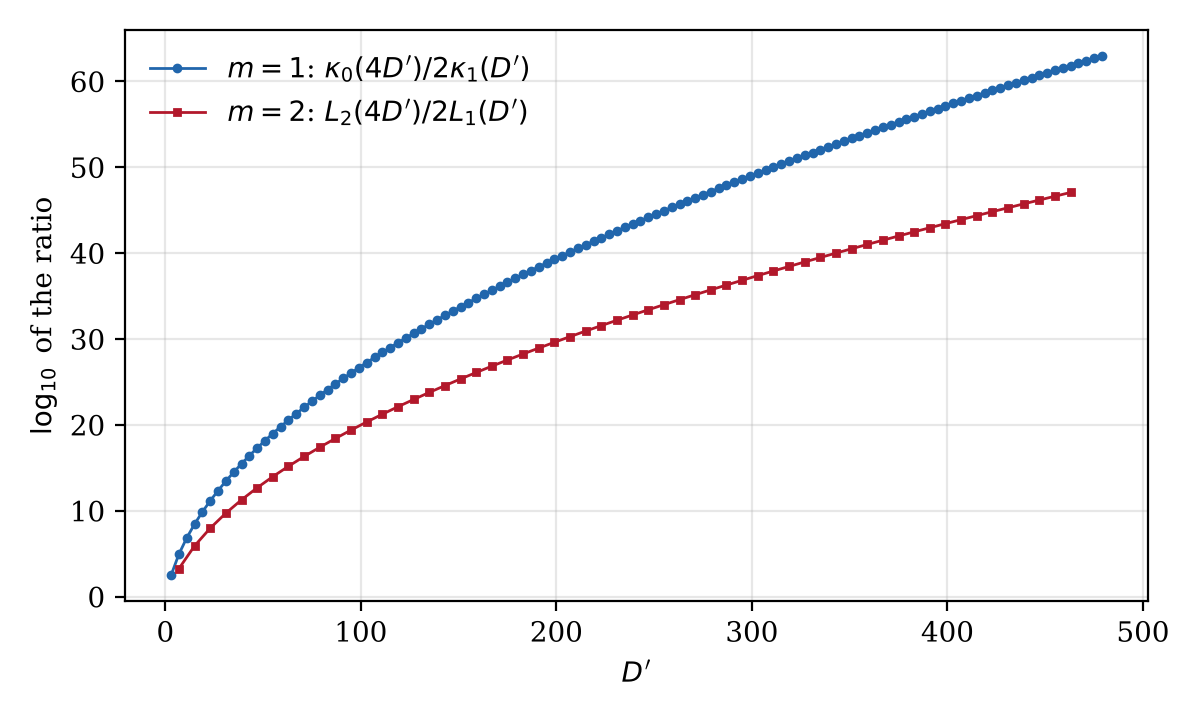
\includegraphics[width=0.78\textwidth]{figures/fig_margins.png}
\caption{The ratio of the two sides of the doubling inequality for $m=1$ (as a function of $D'=4N-1\le479$) and for $m=2$ (as a function of $D'=8j+7\le463$), on a logarithmic scale. The smallest ratios are $325$ at $D'=3$ and $1846$ at $D'=7$; the ratio grows roughly like $\exp(\pi\sqrt{D'})$.}
\label{fig:margins}
\end{figure}

\section{Proof of Theorem~A, and general magnetic charge}\label{sec:proofA}

\begin{proof}[Proof of Theorems~\ref{thm:A} and~\ref{thm:C}]
Theorem~\ref{thm:C} is Theorems~\ref{thm:I1} and~\ref{thm:I2}. For $m\in\{1,2\}$ Bringmann and Murthy proved that $(-1)^{\ell+1}c^F_m(n,\ell)>0$ whenever $4mn-\ell^2>0$ \cite[(3.8)]{BM13}. By Lemma~\ref{lem:allcoeff} this says $d^*(n',\ell',m)>0$ for all $(n',\ell')$ with positive discriminant, which is the hypothesis of Theorem~\ref{thm:B}. Theorem~\ref{thm:C} supplies \eqref{eq:doubling}, and Theorem~\ref{thm:B} gives $d^*_r(Q,P)>0$.
\end{proof}

\begin{example}\label{ex:r2}
Take $r=2$, $m=1$ and $(n,\ell)=(4,2)$, so $\Delta=12$. Then $\ell/2=1$ is odd and
\[
d^*_2=d^*(4,2,1)-2\,d^*(1,1,1)=\kappa(12)-2\kappa(3).
\]
By \eqref{eq:kappa0} and \eqref{eq:kappa1}, $\kappa(3)=25353$ and $\kappa(12)=16491600$, so $d^*_2=16440894>0$. The ratio $\kappa(12)/2\kappa(3)\approx325.2$ is the first row of Table~\ref{tab:I1}, and it is the smallest doubling ratio we have met for any $m$ (Proposition~\ref{prop:numerics}).
\end{example}


\subsection{General magnetic charge}
For $m\ge3$ the positivity of the primitive single-centred indices is not part of this paper, and Theorem~\ref{thm:B} reduces the case of torsion $r$ to it, unconditionally for odd $r$ and through \eqref{eq:doubling} for even $r$. We computed the finite parts $\psi_m^F$ exactly from the product formula for $\Phi_{10}$, by expanding the Fourier--Jacobi coefficients $\psi_m$ and subtracting the Appell--Lerch polar parts, and evaluated $d^*$ at reduced triples through \eqref{eq:DMZ}.

\begin{proposition}[computation]\label{prop:numerics}
The doubling inequality \eqref{eq:doubling} holds for all $2410$ triples $(n',\ell',m)$ with $\ell'$ odd, $|\ell'|\le m$, $m\le199$ and $4\Delta'\le240$; the smallest ratio of the two sides is $325.2$, attained at $(1,\pm1,1)$. The single-centred index \eqref{eq:torsion} is positive for all $6065$ triples with $2\le r\le15$, $|\ell|\le m$ and $\Delta\le240$.
\end{proposition}

\begin{figure}[t]
\centering
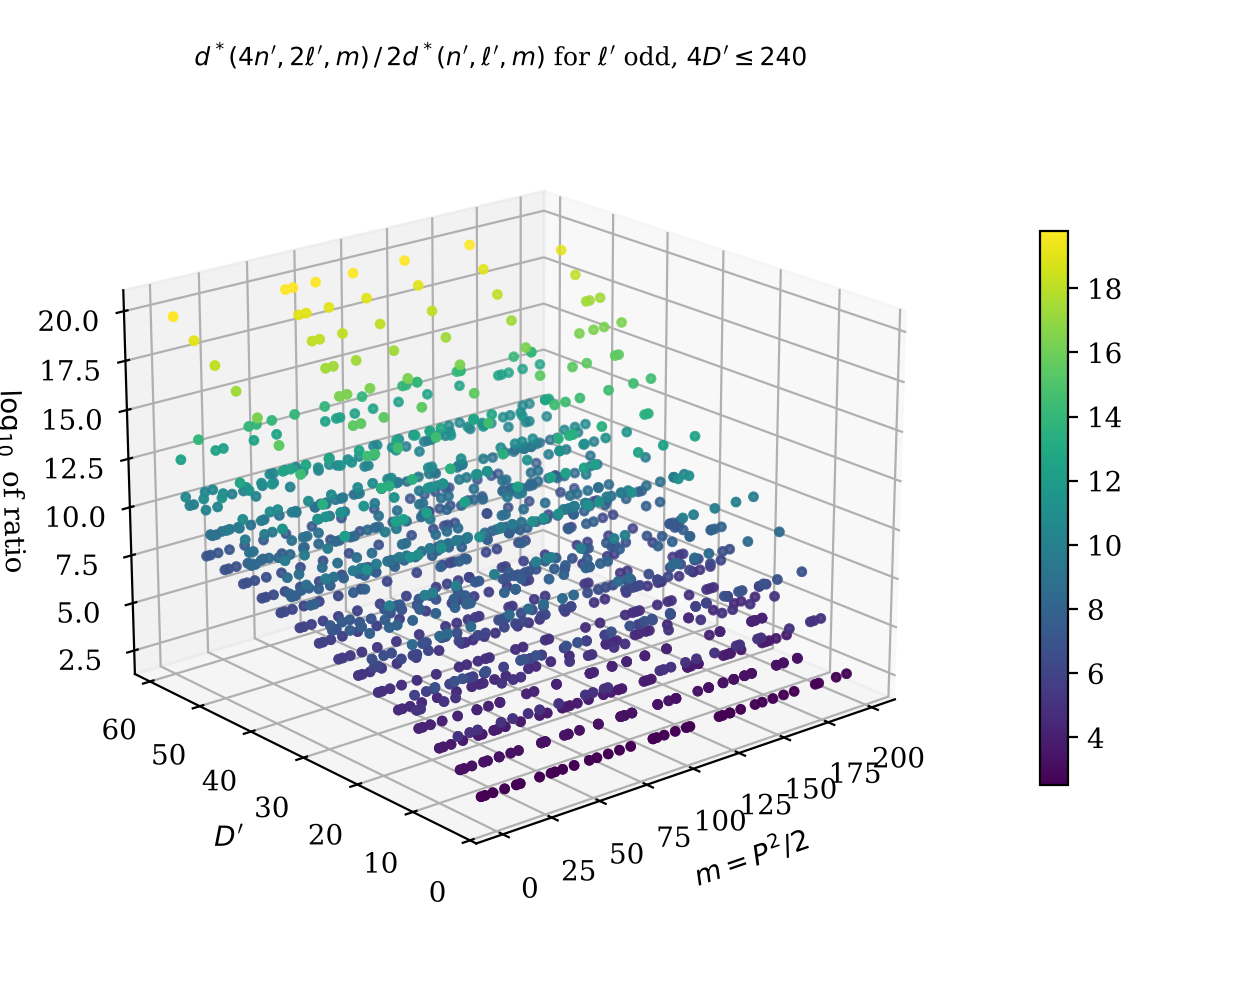
\includegraphics[width=0.72\textwidth]{figures/fig_doubling.png}
\caption{The ratio $d^*(4n',2\ell',m)/2d^*(n',\ell',m)$ on a logarithmic scale for all $2410$ triples of Proposition~\ref{prop:numerics}, plotted against $m$ and $D'=4mn'-\ell'^2$. The ratio depends essentially on $D'$ alone, as expected from the growth $\exp(\pi\sqrt\Delta)$ of the indices.}
\label{fig:doubling}
\end{figure}

Figure~\ref{fig:doubling} suggests that for fixed $D'$ the ratio in \eqref{eq:doubling} hardly depends on $m$. This is what one expects from the Rademacher expansion of the single-centred index, whose leading term depends only on the discriminant \cite{Mur25}, and it suggests that \eqref{eq:doubling} can be proved for all $m$ by the same circle-method estimates that control the primitive indices. We do not pursue this here.

\appendix

\section{\texorpdfstring{The $q$-series for $m=1$ and $m=2$}{The q-series for m=1 and m=2}}\label{app:qseries}

We use the theta functions $\vt_{1,\mu}(\tau,0)$ and $\vt_{2,\mu}(\tau,0)$ of \cite{BM13,EZ85}. For index one,
\[
\theta_\mu(\tau):=\vt_{1,\mu}(\tau,0)=\sum_{r\equiv\mu\,(2)}q^{r^2/4},\qquad \theta_0=\sum_{k\in\ZZ}q^{k^2},\qquad \theta_1=\sum_{r\text{ odd}}q^{r^2/4}=2q^{1/4}T.
\]
Moreover $\theta_1(\tau/2)=\sum_{r\text{ odd}}q^{r^2/8}=2q^{1/8}V$ and $\theta_1(2\tau)=2q^{1/2}T(q^2)$. Writing $\theta'=D\theta$, we have $\theta_1'=\sum_{r\text{ odd}}\frac{r^2}4q^{r^2/4}$, and since $\frac{(2k+1)^2}4=k(k+1)+\frac14$,
\begin{equation}\label{eq:theta1prime}
\theta_1'=2q^{1/4}\big(DT+\tfrac14T\big).
\end{equation}

\subsection{Proof of Proposition~\ref{prop:m1}}
Bringmann and Murthy write \cite[Section~4]{BM13}
\[
\psi_1^F=k_1\vt_{1,1}-k_0\vt_{1,0},\qquad k_1=\frac3\Delta\Big(\frac{E_4\theta_0}{\eta^6}-216\,\mathcal H_1\Big),\qquad k_0=\frac3\Delta\Big(\frac{E_4\theta_1}{\eta^6}+216\,\mathcal H_0\Big),
\]
with $\mathcal H_\mu=\sum_{j\ge0}H(4j+3\mu)q^{j+3\mu/4}$, so that $\mathcal H_0=H_0$ and $\mathcal H_1=q^{3/4}H_1$. The coefficient $c^F_1(n,\ell)$ is the coefficient of $q^{(4n-\ell^2)/4}$ in $k_1$ for $\ell$ odd and in $-k_0$ for $\ell$ even, so $\kappa(D)=(-1)^{\ell+1}c^F_1(n,\ell)$ is the coefficient of $q^{D/4}$ in $k_1$ when $D\equiv3\pmod4$ and in $k_0$ when $D\equiv0\pmod4$.

Using $\eta^{30}=q^{5/4}(q;q)_\infty^{30}$ and $\Delta=q\,(q;q)_\infty^{24}$,
\[
k_0=\frac{3E_4\cdot2q^{1/4}T}{q^{5/4}(q;q)^{30}_\infty}+\frac{648H_0}{q\,(q;q)^{24}_\infty}=q^{-1}\big(6E_4TP_{30}+648H_0P_{24}\big).
\]
The coefficient of $q^{D/4}$ with $D=4N-4$ is the coefficient of $q^{N}$ of the bracket, which is \eqref{eq:kappa0}. Similarly
\[
k_1=3q^{-5/4}E_4\theta_0P_{30}-648\,q^{-1/4}H_1P_{24},
\]
and the coefficient of $q^{D/4}$ with $D=4N-1$, that is of $q^{N-1/4}$, is $3\coef{E_4\theta_0P_{30}}{N+1}-648\coef{H_1P_{24}}{N}$, which is \eqref{eq:kappa1}.

\subsection{Proof of Proposition~\ref{prop:m2}}
Bringmann and Murthy define $\xi_\mu$ by $11E_4\varphi_{-2,1}\varphi_{0,1}-5E_6\varphi_{-2,1}^2=\sum_{\mu=0}^3\xi_\mu\vt_{2,\mu}$ and $F_\mu$ by $\mathcal H|V_2=\sum_\mu F_\mu\vt_{2,\mu}$ \cite[(5.11), (6.1)]{BM13}. By \eqref{eq:psi2F},
\[
\psi_2^F=\sum_\mu\frac{2(\xi_\mu-4800F_\mu)}{3\Delta}\vt_{2,\mu},
\]
so for $\ell\equiv\mu\pmod4$ the index $d^*(n,\ell,2)=(-1)^{\ell+1}c^F_2(n,\ell)$ is the coefficient of $q^{(8n-\ell^2)/8}$ in $\frac23(-1)^{\mu+1}(\xi_\mu-4800F_\mu)/\Delta$. Their formulas \cite[(6.4), (6.5)]{BM13} read
\[
\eta^{12}\xi_1=\tfrac12\theta_1(\tau/2)\,(f_0\theta_0+f_1\theta_1),\qquad -\eta^{12}\xi_2=\theta_1(2\tau)\theta_1f_0+\theta_0(2\tau)\theta_0f_1,
\]
with $f_0=264\theta_1'E_4+g\theta_1$ and $f_1=264\theta_0'E_4+g\theta_0$ \cite[(5.2), (5.3)]{BM13}. By \eqref{eq:theta1prime}, $f_0=2q^{1/4}\big((66T+264DT)E_4+gT\big)=2q^{1/4}\phi_0$, and $f_1=\phi_1$. Hence
\[
f_0\theta_0+f_1\theta_1=2q^{1/4}(\phi_0\theta_0+T\phi_1)=q^{1/4}S,
\]
\[
-\eta^{12}\xi_2=2q^{1/2}T(q^2)\cdot2q^{1/4}T\cdot2q^{1/4}\phi_0+\theta_0(q^2)\theta_0\phi_1=R,
\]
and $\eta^{12}\xi_1=\frac12\cdot2q^{1/8}V\cdot q^{1/4}S=q^{3/8}VS$.

\emph{The case $\mu=2$.} Since $\eta^{36}=q^{3/2}(q;q)^{36}_\infty$, we get $-\xi_2/\Delta=q^{-3/2}RP_{36}$. The class number part is $F_2=\sum_{n\ge1}c(n,2)q^{n-1/2}$ with $c(n,2)=H(8n-4)+2H(2n-1)[n\text{ even}]$ \cite[(5.11)]{BM13}, so $F_2/\Delta=q^{-1/2}C_2P_{24}$ with $C_2=\sum_{k\ge0}c(k+1,2)q^k$. Since $(-1)^{\mu+1}=-1$,
\[
L_2(D)=\tfrac23\Big(\coef{RP_{36}}{D/8+3/2}+4800\coef{C_2P_{24}}{D/8+1/2}\Big),
\]
and $D=4D'$ gives $D/8+3/2=K$ and $D/8+1/2=K-1$, which is \eqref{eq:L2}.

\emph{The case $\mu=1$.} We have $\xi_1/\Delta=q^{3/8-3/2}VSP_{36}=q^{-9/8}VSP_{36}$, and $F_1=\sum_{j\ge1}H(8j-1)q^{j-1/8}$, so $F_1/\Delta=q^{-9/8}H_1'P_{24}$. With $(-1)^{\mu+1}=1$, the coefficient of $q^{D'/8}$ is the coefficient of $q^{(D'+9)/8}=q^M$, which is \eqref{eq:L1}.

\section{Coefficient bounds}\label{app:bounds}

Throughout, $\zeta(3)=1.2020569\ldots$ and $\zeta(5)=1.0369277\ldots$, and we write $e_4(a)=\coef{E_4}a$.

\begin{lemma}\label{lem:g}
$g(0)=-6$ and $g(a)=3024\,\sigma_5(a)-7920\,a\,\sigma_3(a)$ for $a\ge1$. In particular $|g(a)|\le9520.3\,a^5$ for $a\ge1$.
\end{lemma}

\begin{proof}
Ramanujan's identity $DE_4=\frac13(E_2E_4-E_6)$ \cite[Section~5.2]{Zag08} gives $E_2E_4=E_6+3DE_4$, hence $g=5E_6-11E_6-33DE_4=-6E_6-33DE_4$. The coefficient of $q^a$ is $3024\sigma_5(a)-33\cdot240\,a\sigma_3(a)$. Both terms are non-negative, so $|g(a)|$ is at most the larger of them, and $3024\sigma_5(a)\le3024\zeta(5)a^5<3136\,a^5$ while $7920a\sigma_3(a)\le7920\zeta(3)a^4<9520.3\,a^4$.
\end{proof}

\begin{lemma}\label{lem:phi}
For $n\ge1$,
\[
|\phi_0(n)|\le104726\,(1+\sqrt n)\,n^5,\qquad |\phi_1(n)|\le85685\,(1+2\sqrt n)\,n^5,
\]
and $\phi_0(0)=60$, $\phi_1(0)=-6$.
\end{lemma}

\begin{proof}
The coefficient of $q^n$ in $\phi_0$ is $\sum_{t}\big((66+264t)e_4(n-t)+g(n-t)\big)$ over $t=k(k+1)\le n$ with $k\ge0$; there are at most $1+\sqrt n$ such $t$. If $a=n-t\ge1$, then $(66+264t)e_4(a)\le330n\cdot288.5n^3=95205n^4$ and $|g(a)|\le9520.3n^5$, so the term is at most $104725.3\,n^5$. If $t=n$, the term is $66+264n-6\le330n$. This gives the bound for $\phi_0$, and $\phi_0(0)=66-6$.

Similarly the coefficient of $q^n$ in $\phi_1$ is $\sum_{k\in\ZZ,\,k^2\le n}\big(264k^2e_4(n-k^2)+g(n-k^2)\big)$, with at most $1+2\sqrt n$ terms, each bounded by $264n\cdot288.5n^3+9520.3n^5\le85685n^5$ when $n-k^2\ge1$ and by $264n$ when $k^2=n$. Finally $\phi_1(0)=g(0)=-6$.
\end{proof}

\begin{lemma}\label{lem:Sbound}
For $n\ge1$, $|S(n)|\le380822\,(1+\sqrt n)(1+2\sqrt n)\,n^5$, and for $i\ge1$, $\sigma(i)\le5.5164\cdot10^6\,i^{13/2}$.
\end{lemma}

\begin{proof}
We have $S(n)=2\sum_{k\in\ZZ,\,k^2\le n}\phi_0(n-k^2)+2\sum_{k\ge0,\,k(k+1)\le n}\phi_1(n-k(k+1))$. The bounds of Lemma~\ref{lem:phi} increase with $n$ and also dominate $|\phi_0(0)|=60$ and $|\phi_1(0)|=6$, so
\begin{align*}
|S(n)|&\le2(1+2\sqrt n)\cdot104726(1+\sqrt n)n^5+2(1+\sqrt n)\cdot85685(1+2\sqrt n)n^5\\
&=380822(1+\sqrt n)(1+2\sqrt n)n^5.
\end{align*}
Next $\sigma(i)=\sum_{k\ge0,\,k(k+1)/2\le i}S(i-k(k+1)/2)$ has at most $1+\sqrt{2i}$ terms, each at most $380822(1+\sqrt i)(1+2\sqrt i)i^5$ in absolute value (the term $S(0)=108$ included). For $i\ge1$, $(1+\sqrt{2i})(1+\sqrt i)(1+2\sqrt i)\le(1+\sqrt2)\cdot2\cdot3\,i^{3/2}<14.4854\,i^{3/2}$, and $380822\cdot14.4854<5.5164\cdot10^6$.
\end{proof}

\begin{remark}
The constants are far from optimal. The largest value of $|g(a)|/a^5$ is $4896$, at $a=1$, and the largest value of $|S(n)|/((1+2\sqrt n)^2n^5)$ for $1\le n\le400$ is below $1500$. Sharper constants would shorten the tables of Appendix~\ref{app:tables} but are not needed.
\end{remark}

\section{Exact values}\label{app:tables}

All values below are exact integers, computed from Propositions~\ref{prop:m1} and~\ref{prop:m2} with $H(N)$ obtained by counting reduced binary quadratic forms. Every value that also appears in the coefficient tables of \cite[Appendix~A]{BM13} agrees with it.

\begin{table}[h]
\centering
\small
\begin{tabular}{rr}
\toprule
$\ell$ & $(-1)^{\ell+1}c^F_2(1,\ell)=(-1)^{\ell+1}c^F_1(2,\ell)$\\
\midrule
$0$ & $1127472$\\
$\pm1$ & $561576$\\
$\pm2$ & $50064$\\
\bottomrule
\end{tabular}
\caption{The coefficients used in the proof of Lemma~\ref{lem:allcoeff}.}
\label{tab:prim}
\end{table}

\begin{table}[h]
\centering
\small
\begin{tabular}{rrrr}
\toprule
$N$ & $D'=4N-1$ & $\kappa(16N-4)$ & $\kappa(4N-1)$\\
\midrule
1 & 3 & 16491600 & 25353\\
2 & 7 & 101777516400 & 561576\\
3 & 11 & 120407289152016 & 8533821\\
4 & 15 & 56968670205288432 & 100390104\\
5 & 19 & 14565081067453280016 & 977183520\\
6 & 23 & 2367012428714552500416 & 8203464720\\
7 & 27 & 270323327028195388932480 & 61077837780\\
8 & 31 & 23209296513809277674799504 & 411421124040\\
9 & 35 & 1571840916640008683741660160 & 2544746970243\\
\bottomrule
\end{tabular}
\caption{Inequality \eqref{eq:I1} for $1\le N\le9$.}
\label{tab:I1}
\end{table}

\begin{table}[h]
\centering
\small
\begin{tabular}{rrrr}
\toprule
$j$ & $D'=8j+7$ & $L_2(4D')$ & $L_1(D')$\\
\midrule
0 & 7 & 2073849984 & 561576\\
1 & 15 & 30312295881600 & 18458000\\
2 & 23 & 73625812211910912 & 392427528\\
3 & 31 & 65440347323367281280 & 6216536784\\
4 & 39 & 29554733204711345826304 & 79330416536\\
5 & 47 & 8102515491418262427894144 & 855667882536\\
\bottomrule
\end{tabular}
\caption{Inequality \eqref{eq:I2} for $0\le j\le5$.}
\label{tab:I2}
\end{table}

\section*{Declarations}

\noindent\textbf{Data availability.} The programs that compute the $q$-series of Propositions~\ref{prop:m1} and~\ref{prop:m2}, check every constant of Lemmas~\ref{lem:m1bounds}, \ref{lem:m2bounds} and Appendix~\ref{app:bounds}, produce Tables~\ref{tab:prim}--\ref{tab:I2} and Proposition~\ref{prop:numerics}, and draw the figures are archived at \cite{Bha26}.

\smallskip\noindent\textbf{Funding.} None.

\smallskip\noindent\textbf{Conflicts of interest.} None.

\begin{thebibliography}{99}

\bibitem{BBS23} D.~Bhattacharjee, P.~Bose, P.~Samal, \emph{Ramanujan $\tau$-function and its relationship with $PSL(2,\mathbb Z)$ for $\mathcal L_{24}(\tau)^{+,E}$}, Research Square (2023). doi:10.21203/rs.3.rs-2796280/v1

\bibitem{Bha22} D.~Bhattacharjee, \emph{Generalization of quartic and quintic Calabi--Yau manifolds fibered by polarized K3 surfaces}, Research Square (2022). doi:10.21203/rs.3.rs-1965255/v1

\bibitem{Bha26} D.~Bhattacharjee, \emph{Code and data for: Positive black hole degeneracies for dyons of higher torsion}, version v1.0.0, Zenodo (2026). doi:\zenodoDOI

\bibitem{BM13} K.~Bringmann, S.~Murthy, \emph{On the positivity of black hole degeneracies in string theory}, Commun. Number Theory Phys. \textbf{7} (2013), 15--56. doi:10.4310/CNTP.2013.v7.n1.a2

\bibitem{BN26} D.~Bhattacharjee, P.~Nandi, \emph{Enriques and Kummer surfaces arising from K3 involutions}, Preprints (2026). doi:10.20944/preprints202602.0098.v1

\bibitem{BSS08a} S.~Banerjee, A.~Sen, Y.~K.~Srivastava, \emph{Partition functions of torsion $>1$ dyons in heterotic string theory on $T^6$}, J. High Energy Phys. \textbf{2008}, no.~5 (2008), 098. doi:10.1088/1126-6708/2008/05/098

\bibitem{BSS08b} S.~Banerjee, A.~Sen, Y.~K.~Srivastava, \emph{Generalities of quarter BPS dyon partition function and dyons of torsion two}, J. High Energy Phys. \textbf{2008}, no.~5 (2008), 101. doi:10.1088/1126-6708/2008/05/101

\bibitem{BSS09} S.~Banerjee, A.~Sen, Y.~K.~Srivastava, \emph{Genus two surface and quarter BPS dyons: the contour prescription}, J. High Energy Phys. \textbf{2009}, no.~3 (2009), 151. doi:10.1088/1126-6708/2009/03/151

\bibitem{CD21} A.~Chattopadhyaya, J.~R.~David, \emph{Horizon states and the sign of their index in $\mathcal N=4$ dyons}, J. High Energy Phys. \textbf{2021}, no.~3 (2021), 106. doi:10.1007/JHEP03(2021)106

\bibitem{CV08} M.~C.~N.~Cheng, E.~P.~Verlinde, \emph{Wall crossing, discrete attractor flow and Borcherds algebra}, SIGMA \textbf{4} (2008), 068. doi:10.3842/SIGMA.2008.068

\bibitem{DGM11} A.~Dabholkar, J.~Gomes, S.~Murthy, \emph{Counting all dyons in $\mathcal N=4$ string theory}, J. High Energy Phys. \textbf{2011}, no.~5 (2011), 059. doi:10.1007/JHEP05(2011)059

\bibitem{DGMS11} A.~Dabholkar, J.~Gomes, S.~Murthy, A.~Sen, \emph{Supersymmetric index from black hole entropy}, J. High Energy Phys. \textbf{2011}, no.~4 (2011), 034. doi:10.1007/JHEP04(2011)034

\bibitem{DVV97} R.~Dijkgraaf, E.~Verlinde, H.~Verlinde, \emph{Counting dyons in $N=4$ string theory}, Nucl. Phys. B \textbf{484} (1997), 543--561. doi:10.1016/S0550-3213(96)00640-2

\bibitem{EZ85} M.~Eichler, D.~Zagier, \emph{The Theory of Jacobi Forms}, Progress in Mathematics \textbf{55}, Birkh\"auser, Boston, 1985. doi:10.1007/978-1-4684-9162-3

\bibitem{GN97} V.~A.~Gritsenko, V.~V.~Nikulin, \emph{Siegel automorphic form corrections of some Lorentzian Kac--Moody Lie algebras}, Amer. J. Math. \textbf{119} (1997), 181--224. doi:10.1353/ajm.1997.0002

\bibitem{HZ76} F.~Hirzebruch, D.~Zagier, \emph{Intersection numbers of curves on Hilbert modular surfaces and modular forms of Nebentypus}, Invent. Math. \textbf{36} (1976), 57--113. doi:10.1007/BF01390005

\bibitem{Mur25} S.~Murthy, \emph{Black holes and modular forms in string theory}, in: Oxford Research Encyclopedia of Physics, Oxford University Press, 2025. doi:10.1093/acrefore/9780190871994.013.65

\bibitem{SBBT26} R.~Sadhu, D.~Bhattacharjee, S.~Bhattacharya, S.~N.~Thakur, \emph{$E_8\times E_8$ heterotic gravity and M-theory}, SSRN (2026). doi:10.2139/ssrn.6326718

\bibitem{Sen07} A.~Sen, \emph{Walls of marginal stability and dyon spectrum in $\mathcal N=4$ supersymmetric string theories}, J. High Energy Phys. \textbf{2007}, no.~5 (2007), 039. doi:10.1088/1126-6708/2007/05/039

\bibitem{Sen08} A.~Sen, \emph{Black hole entropy function, attractors and precision counting of microstates}, Gen. Relativ. Gravit. \textbf{40} (2008), 2249--2431. doi:10.1007/s10714-008-0626-4

\bibitem{Sen11} A.~Sen, \emph{How do black holes predict the sign of the Fourier coefficients of Siegel modular forms?}, Gen. Relativ. Gravit. \textbf{43} (2011), 2171--2183. doi:10.1007/s10714-011-1175-9

\bibitem{SSY06} D.~Shih, A.~Strominger, X.~Yin, \emph{Recounting dyons in $\mathcal N=4$ string theory}, J. High Energy Phys. \textbf{2006}, no.~10 (2006), 087. doi:10.1088/1126-6708/2006/10/087

\bibitem{Zag08} D.~Zagier, \emph{Elliptic modular forms and their applications}, in: The 1-2-3 of Modular Forms, Universitext, Springer, Berlin, 2008, 1--103. doi:10.1007/978-3-540-74119-0\_1

\end{thebibliography}

\end{document}
